%%%%%%%%%%%%%%%%%%%%%%%%%%%%%%%%%%%%%%%%%
% Masters/Doctoral Thesis 
% LaTeX Template
% Version 2.4 (22/11/16)
%
% This template has been downloaded from:
% http://www.LaTeXTemplates.com
%
% Version 2.x major modifications by:
% Vel (vel@latextemplates.com)
%
% This template is based on a template by:
% Steve Gunn (http://users.ecs.soton.ac.uk/srg/softwaretools/document/templates/)
% Sunil Patel (http://www.sunilpatel.co.uk/thesis-template/)
%
% Template license:
% CC BY-NC-SA 3.0 (http://creativecommons.org/licenses/by-nc-sa/3.0/)
%
%%%%%%%%%%%%%%%%%%%%%%%%%%%%%%%%%%%%%%%%%

%----------------------------------------------------------------------------------------
%	PACKAGES AND OTHER DOCUMENT CONFIGURATIONS
%----------------------------------------------------------------------------------------

\documentclass[
11pt, % The default document font size, options: 10pt, 11pt, 12pt
%oneside, % Two side (alternating margins) for binding by default, uncomment to switch to one side
english, % ngerman for German
singlespacing, % Single line spacing, alternatives: onehalfspacing or doublespacing
%draft, % Uncomment to enable draft mode (no pictures, no links, overfull hboxes indicated)
%nolistspacing, % If the document is onehalfspacing or doublespacing, uncomment this to set spacing in lists to single
%liststotoc, % Uncomment to add the list of figures/tables/etc to the table of contents
%toctotoc, % Uncomment to add the main table of contents to the table of contents
%parskip, % Uncomment to add space between paragraphs
%nohyperref, % Uncomment to not load the hyperref package
headsepline, % Uncomment to get a line under the header
%chapterinoneline, % Uncomment to place the chapter title next to the number on one line
%consistentlayout, % Uncomment to change the layout of the declaration, abstract and acknowledgements pages to match the default layout
]{MastersDoctoralThesis} % The class file specifying the document structure

\usepackage[utf8]{inputenc} % Required for inputting international characters
\usepackage[T1]{fontenc} % Output font encoding for international characters

\usepackage{palatino} % Use the Palatino font by default

\usepackage[backend=bibtex,style=authoryear,natbib=true]{biblatex} % Use the bibtex backend with the authoryear citation style (which resembles APA)

\addbibresource{example.bib} % The filename of the bibliography

\usepackage[autostyle=true]{csquotes} % Required to generate language-dependent quotes in the bibliography

%----------------------------------------------------------------------------------------
%	MARGIN SETTINGS
%----------------------------------------------------------------------------------------

\geometry{
	paper=a4paper, % Change to letterpaper for US letter
	inner=2.5cm, % Inner margin
	outer=3.8cm, % Outer margin
	bindingoffset=.5cm, % Binding offset
	top=1.5cm, % Top margin
	bottom=1.5cm, % Bottom margin
	%showframe, % Uncomment to show how the type block is set on the page
}

%----------------------------------------------------------------------------------------
%	THESIS INFORMATION
%----------------------------------------------------------------------------------------

\thesistitle{Thesis Title} % Your thesis title, this is used in the title and abstract, print it elsewhere with \ttitle
\supervisor{Ståle\textsc{Walderhaug}} % Your supervisor's name, this is used in the title page, print it elsewhere with \supname
\examiner{} % Your examiner's name, this is not currently used anywhere in the template, print it elsewhere with \examname
\degree{Doctor of Philosophy} % Your degree name, this is used in the title page and abstract, print it elsewhere with \degreename
\author{Andrea \textsc{Spreafico}} % Your name, this is used in the title page and abstract, print it elsewhere with \authorname
\addresses{} % Your address, this is not currently used anywhere in the template, print it elsewhere with \addressname

\subject{Biological Sciences} % Your subject area, this is not currently used anywhere in the template, print it elsewhere with \subjectname
\keywords{} % Keywords for your thesis, this is not currently used anywhere in the template, print it elsewhere with \keywordnames
\university{\href{http://www.university.com}{University Name}} % Your university's name and URL, this is used in the title page and abstract, print it elsewhere with \univname
\department{\href{http://department.university.com}{Department or School Name}} % Your department's name and URL, this is used in the title page and abstract, print it elsewhere with \deptname
\group{\href{http://researchgroup.university.com}{Research Group Name}} % Your research group's name and URL, this is used in the title page, print it elsewhere with \groupname
\faculty{\href{http://faculty.university.com}{Faculty Name}} % Your faculty's name and URL, this is used in the title page and abstract, print it elsewhere with \facname

\AtBeginDocument{
\hypersetup{pdftitle=\ttitle} % Set the PDF's title to your title
\hypersetup{pdfauthor=\authorname} % Set the PDF's author to your name
\hypersetup{pdfkeywords=\keywordnames} % Set the PDF's keywords to your keywords
}

\begin{document}

\frontmatter % Use roman page numbering style (i, ii, iii, iv...) for the pre-content pages

\pagestyle{plain} % Default to the plain heading style until the thesis style is called for the body content

%----------------------------------------------------------------------------------------
%	TITLE PAGE
%----------------------------------------------------------------------------------------

\begin{titlepage}
\begin{center}

\vspace*{.06\textheight}
{\scshape\LARGE \univname\par}\vspace{1.5cm} % University name
\textsc{\Large Doctoral Thesis}\\[0.5cm] % Thesis type

\HRule \\[0.4cm] % Horizontal line
{\huge \bfseries \ttitle\par}\vspace{0.4cm} % Thesis title
\HRule \\[1.5cm] % Horizontal line
 
\begin{minipage}[t]{0.4\textwidth}
\begin{flushleft} \large
\emph{Author:}\\
\href{http://www.johnsmith.com}{\authorname} % Author name - remove the \href bracket to remove the link
\end{flushleft}
\end{minipage}
\begin{minipage}[t]{0.4\textwidth}
\begin{flushright} \large
\emph{Supervisor:} \\
\href{http://www.jamessmith.com}{\supname} % Supervisor name - remove the \href bracket to remove the link  
\end{flushright}
\end{minipage}\\[3cm]
 
\vfill

\large \textit{A thesis submitted in fulfillment of the requirements\\ for the degree of \degreename}\\[0.3cm] % University requirement text
\textit{in the}\\[0.4cm]
\groupname\\\deptname\\[2cm] % Research group name and department name
 
\vfill

{\large \today}\\[4cm] % Date
%\includegraphics{Logo} % University/department logo - uncomment to place it
 
\vfill
\end{center}
\end{titlepage}

%----------------------------------------------------------------------------------------
%	DECLARATION PAGE
%----------------------------------------------------------------------------------------

\begin{declaration}
\addchaptertocentry{\authorshipname} % Add the declaration to the table of contents
\noindent I, \authorname, declare that this thesis titled, \enquote{\ttitle} and the work presented in it are my own. I confirm that:

\begin{itemize} 
\item This work was done wholly or mainly while in candidature for a research degree at this University.
\item Where any part of this thesis has previously been submitted for a degree or any other qualification at this University or any other institution, this has been clearly stated.
\item Where I have consulted the published work of others, this is always clearly attributed.
\item Where I have quoted from the work of others, the source is always given. With the exception of such quotations, this thesis is entirely my own work.
\item I have acknowledged all main sources of help.
\item Where the thesis is based on work done by myself jointly with others, I have made clear exactly what was done by others and what I have contributed myself.\\
\end{itemize}
 
\noindent Signed:\\
\rule[0.5em]{25em}{0.5pt} % This prints a line for the signature
 
\noindent Date:\\
\rule[0.5em]{25em}{0.5pt} % This prints a line to write the date
\end{declaration}

\cleardoublepage

%----------------------------------------------------------------------------------------
%	QUOTATION PAGE
%----------------------------------------------------------------------------------------

\vspace*{0.2\textheight}

\noindent\enquote{\itshape Thanks to my solid academic training, today I can write hundreds of words on virtually any topic without possessing a shred of information, which is how I got a good job in journalism.}\bigbreak

\hfill Dave Barry

%----------------------------------------------------------------------------------------
%	ABSTRACT PAGE
%----------------------------------------------------------------------------------------

\begin{abstract}
\addchaptertocentry{\abstractname} % Add the abstract to the table of contents
The Thesis Abstract is written here (and usually kept to just this page). The page is kept centered vertically so can expand into the blank space above the title too\ldots
\end{abstract}

%----------------------------------------------------------------------------------------
%	ACKNOWLEDGEMENTS
%----------------------------------------------------------------------------------------

\begin{acknowledgements}
\addchaptertocentry{\acknowledgementname} % Add the acknowledgements to the table of contents
The acknowledgments and the people to thank go here, don't forget to include your project advisor\ldots
\end{acknowledgements}

%----------------------------------------------------------------------------------------
%	LIST OF CONTENTS/FIGURES/TABLES PAGES
%----------------------------------------------------------------------------------------

\tableofcontents % Prints the main table of contents

\listoffigures % Prints the list of figures

\listoftables % Prints the list of tables

%----------------------------------------------------------------------------------------
%	ABBREVIATIONS
%----------------------------------------------------------------------------------------

\begin{abbreviations}{ll} % Include a list of abbreviations (a table of two columns)

\textbf{LAH} & \textbf{L}ist \textbf{A}bbreviations \textbf{H}ere\\
\textbf{WSF} & \textbf{W}hat (it) \textbf{S}tands \textbf{F}or\\

\end{abbreviations}

%----------------------------------------------------------------------------------------
%	PHYSICAL CONSTANTS/OTHER DEFINITIONS
%----------------------------------------------------------------------------------------

\begin{constants}{lr@{${}={}$}l} % The list of physical constants is a three column table

% The \SI{}{} command is provided by the siunitx package, see its documentation for instructions on how to use it

Speed of Light & $c_{0}$ & \SI{2.99792458e8}{\meter\per\second} (exact)\\
%Constant Name & $Symbol$ & $Constant Value$ with units\\

\end{constants}

%----------------------------------------------------------------------------------------
%	SYMBOLS
%----------------------------------------------------------------------------------------

\begin{symbols}{lll} % Include a list of Symbols (a three column table)

$a$ & distance & \si{\meter} \\
$P$ & power & \si{\watt} (\si{\joule\per\second}) \\
%Symbol & Name & Unit \\

\addlinespace % Gap to separate the Roman symbols from the Greek

$\omega$ & angular frequency & \si{\radian} \\

\end{symbols}

%----------------------------------------------------------------------------------------
%	DEDICATION
%----------------------------------------------------------------------------------------

\dedicatory{For/Dedicated to/To my\ldots} 

%----------------------------------------------------------------------------------------
%	THESIS CONTENT - CHAPTERS
%----------------------------------------------------------------------------------------

\mainmatter % Begin numeric (1,2,3...) page numbering

\pagestyle{thesis} % Return the page headers back to the "thesis" style

% Include the chapters of the thesis as separate files from the Chapters folder
% Uncomment the lines as you write the chapters

%*******10********20********30********40********50********60********70********80

\chap{Introduction}


\section{Aim of the study}
Every single day in the world is produced a huge amount of data: some of this data, if they are analyzed and interpreted in the right away, could provide useful informations.\\
If we watch for example at the Aquaculture business in Norway is produced a big amount of data about every single locality or about national statistcs, but most of the time this data are not analyzed and difficult to understand.\\
The main purposes of this thesis are basically to test and show:
\begin{itemize} 
 \item 	Data potential in Aquaculture business in Norway through a system for analyzing and displaying data, in order to help the companies related with Aquaculture to improve their operations thanks to the analysis results.
 \item 	Python potential in data science, in order to show the people how it works and what you could do using it.
 \end{itemize}
For achieve the goals reported above, this thesis will provide:
\begin{itemize} 
 \item 	Implementation and description of a procedure that can be used for make a Python system able to do an initial analysis of  big datasets and also to display the obtained results.
 \item Implementation and description of a procedure that can be used for make a system implemented in Python able to predict future’s values using a regression model.
 \item List of possible implementation for further uses of machine learning algorithms and regression model.
 
 \end{itemize}

\newpage
\section{Initial Goals}

\textbf{1) Collect as much data about aquaculture in Norway as possible.}\\
- Is possible to obtain data about aquaculture general statistics in Norway?\\
- Is possible to obtain data about aquaculture of single locations in Norway?

 
\textbf{2) Increase accessibility and availability of the data.}\\
- Is that possible to create a unique dataset that contains all the data previous collected?\\
- Is the total dataset easier to access and read the new dataset structure compared with original single sources?

 
\textbf{3) Analyze and display the data.}\\
- Is that possible to provide a general analysis and displaying of data about Norwegian aquaculture reported in the dataset?\\
- Is that possible to use Python for analyzing and displaying the data?\\
	- Is Python a good programming language for data analysis and displaying?\\
	- Does Python give the possibility to create analysis systems in easy way?
- Are the obtained graphics allowing to comprehend information quickly?\\
- Are the obtained graphics allowing to identify relationships and patterns in a easy way?\\
- Are the obtained graphics allowing to identify historic and future trend line?\\
- Are the obtained informations (such as correlation coeff, trend line equations,..)reported in documents ready to be reused in the future?
 
\textbf{4) Extract information from the data.}	\\
- Is the aquaculture business in Norway growing? \\
- More in the specific, which parameters are increasing and how fast? \\
- Is that possible to have a trend line about the data? \\
- Is that possible to find some correlations between the data in input and display them? \\
- Are that data influenced from external parameters? Such as weather, news, people ideas..

 
\textbf{5) Prediction of values about the data.}\\
- Is that possible to predict some of the data that we own?\\
		- Would it be useful to have the possibility of forecasting some future data?\\
		- Which kind of data might be the most useful to know for people into the Aquaculture field?\\
-Test and describe time series predictions utility in Python.\\
		- Is Python a good way for time series prediction systems implementation?\\
		- Does it give the possibility to have accurate results?\\
		- Is that good for let the people get some experience with machine learning field?


\textbf{6) Recommendations to future work and extra ideas.}\\
- Is that possible to let the informations collected before be available like a service?\\
		- Is that possible to provide the analysis and prediction systems like a service?\\
		- Is that possible to let the data displaying dynamic instead of static?\\






%%*******10********20********30********40********50********60********70********80

\chap{Background Theory} 

The background theory required for implement this thesis work could be basically divided into 4 main areas:
\begin{itemize}
\item Data science
\item Aquaculture in Norway
\item Machine Learning
\item Python
\end{itemize}

Could be very useful to give some basic definitions and explanations about the topics written just above and then try to get some more specific informations during the course of this thesis.

\newpage
\section{Data science}
It's really important to have a general idea about what "Data Science" means since this thesis procedure is strongly based on the classic Data Science Process.
We can define Data Science like a "concept to unify statistics, data analysis and their related methods" in order to "understand and analyze actual phenomena" with data.
It includes theories drawn from many field within the broad areas of mathematics, statistics, information science and computer science.

In the computer science area in particular the subdomains of machine learning, classification, cluster analysis, data mining, databases, and visualization.
The follow image represents the "Blitzstein and Pfister's framework" and provides a clear overview of the topic.

\begin{figure}[h]
    \centering
    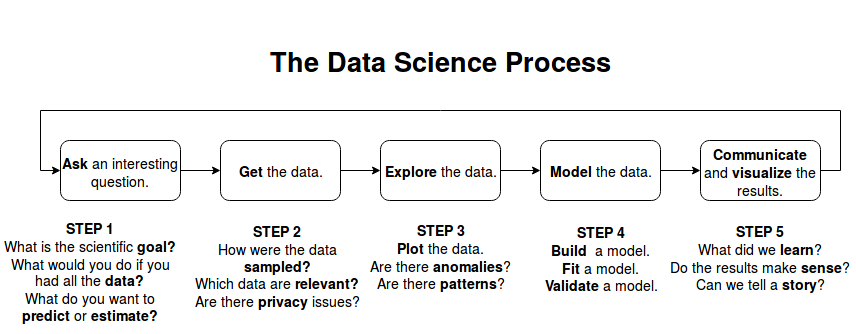
\includegraphics[trim=0cm 0cm 0cm 0cm, clip=true, width=1\textwidth,natwidth=819,natheight=321]{Files/Data_Science_Process.png}
    \caption[Data science process]{Data science process}
    \label{fig: Data_science}
\end{figure}

\section{Aquaculture in Norway}
Aquaculture, also known as aquafarming, is the farming of fish, crustaceans, molluscs, aquatic plants, algae, and other aquatic organisms.

Aquaculture would be the future of fish:
In 2030, according to the World Bank, aquaculture will supply:
\begin{itemize}
\item 93.6 Million tonnes of fish per year
\item 25 percent less wild fish will be available
\item 62 percent of the fish we eat will come from farms
\end{itemize}


\section{Machine learning}
This subfield of computer science gives "computers the ability to learn without being explicitly programmed". \\Evolved from the study of pattern recognition and computational learning theory in artificial intelligence, machine learning explores the study and construction of algorithms that can learn from and make predictions on data.

There are several machine learning algorithm, each one of them is used for a different purpose.The following picture gives a general idea about which categories of algorithms are used and some specific types.


\subsection{Time Series analysis and predictions}
Time Series forecasting is an important area of machine learning, but that is often neglected.

Is that important mainly beause there are so many prediction problems that involve a time component, and these problems are neglected because it is this time component that makes time series problems more difficult to handle.

" A time series is a sequence of observations taken sequentially in time. "
Quoted — Page 1, Time Series Analysis: Forecasting and Control.

Classic example of a time series dataset:\\ 		
Time \#1, observation\\
Time \#2, observation\\
Time \#3, observation

There are different goals depending on wheter we are interested in understanding a dataset or making predictions.

Understanding a dataset is called time series analysis and it can helps to make better prediction, but sometimes it's not required and can result in a large of technocal investment in time and expertise.

Making predictions could be called time series forecasting and it involves taking models fit on historical data and using them to predict future observations.

Information Source: http://machinelearningmastery.com/time-series-forecasting/
\section{Python}


 
%%*******10********20********30********40********50********60********70********80

% For all chapters, use the newdefined chap{} instead of chapter{}
% This will make the text at the top-left of the page be the same as the chapter

\chap{Development Method}

In order to achieve the problem reported in the introduction, has been developed an easy but clear plan (how you can see in the follow picture 3.1).\\

\begin{figure}[h]
    \centering
    \includegraphics[trim=0cm 0cm 0cm 0cm, clip=true, width=0.65\textwidth,natwidth=610,natheight=642]{Files/PlanChart.png}
    \caption[Plan flow chart]{Plan flow chart}
    \label{fig: Plan_Flow_Chart}
\end{figure}

\newpage
\textbf{1st Phase: Data collection}
During this phase the most important thing is to gather as much as possible data, 	but they must be as much as possible reliable and useful they are going to be indispensable for the next phases and in particular the final result and conclusion.
The data’s reliability and utility mainly depend by the kind of sources where you’re able to mine.

\textbf{2nd Phase: Dataset creation}
During this phase you should customize the unstructured data that you collected in the first phase. This data’s customizing has the main purpose to let the data structure follow some kind of setting and standard needed in the system that will be implemented later on.
Part of this phase has to be done meanwhile you’re working on the successive phase, since you’re going to discover a lot of needed setting and standard once you’re trying to feed the system.

\textbf{3rd Phase: Data analysis}
During this phase the first thing that you’re going to do is to decide some kind of analysis results that you would like to have.
Once you decided which kind of results you might reach, you will start with the analysis system implementation and then for the predictions system.

	\qquad \textbf {3.1rd Phase – Initial data analysis system:}

	\qquad \textbf {3.2rd Phase – Data prediction system:}

\textbf{4th Phase: Data displaying}
This is the last but not least phase since displaying some information in a easy-read mode sometimes is very difficult.
During this phase the main purpose will be to find a way to display the analysis results in a way that could be easily understand.

	\qquad \textbf {4.1th Phase - Initial analysis results displaying}
	
	\qquad \textbf {4.2th Phase - Prediction results displaying}
\newpage 
%\chap{Implementation}

\lstset{
language=Python,
backgroundcolor = \color{Ivory},
basicstyle=\ttfamily,
otherkeywords={self},             
keywordstyle=\ttfamily\color{blue!90!black},
keywords=[2]{True,False},
keywords=[3]{ttk},
keywordstyle={[2]\ttfamily\color{yellow!80!orange}},
keywordstyle={[3]\ttfamily\color{red!80!orange}},
emph={MyClass,__init__},          
emphstyle=\ttfamily\color{red!80!black},    
stringstyle=\color{green!80!black},
showstringspaces=false            
}

\hypersetup{
    colorlinks=true,
    linkcolor=blue,
    filecolor=magenta,      
    urlcolor=cyan,
}
Total implementation link for Experiment 1 : \\
\hyperlink{https://github.com/Sprea22/Data_Analyzer_Python}{https://github.com/Sprea22/Data\_Analyzer\_Python}

Total implementation link for Experiment 2 : \\
\url{}

(INSTRUCTION FOR DOWNLOAD AND USE FROM GITHUB)

\newpage
\section{1st Phase: Data collection}
During this phase is important to be sure to have all the data that we are going to need. During this particular implementation we need the 7 input dataset written above in the "Dataset structure" section, and below here you can find the link of the website where you can download all the needed datasets for this example.

Datasets downloads website:\\ 
\hyperlink{http://www.fiskeridir.no/Akvakultur/Statistikk-akvakultur/Biomassestatistikk} {http://www.fiskeridir.no/Akvakultur/Statistikk-akvakultur/Biomassestatistikk} \\

The datasets that you can download on this website are in a different format than the one we will need, but for better understand the meaning of the data are useful since are in XLSX format, splitted in clear tables and well commented (only in norwegian).

\subsection{Data sources}
\subsection{Data description and validation}

\newpage
\section{2nd Phase: Dataset creation}
\subsection{Processing the data}
Once we have all the "row" data we can start to setup the dataset that we will need for this system. 
First of all we will use the format CSV for the new datasets instead of XLSX.
Then we need to create three different "standards" of each input dataset. The reason of this requirement is that using the python library for some kind of analysis is easier to read the data in a particular format instead of reading the data always in the normal CSV standard and then edit and handle it later through the code.
Following are reported the needed standards.

\begin{itemize}
\item Normal CSV standard (Standard\_N)
\begin{table}[ht] 
    \centering 
    \begin{tabular}{ | l | l |}
        \hline
       	Month & Input\_Name\\ \hline
        January\_2005 & Value1 \\ \hline
        February\_2005 & Value2\\ \hline
        March\_2005 & Value3\\ \hline
        ... & ...\\ \hline
        November\_2016 & Value143\\ \hline
        December\_2016 & Value144\\ \hline
    \end{tabular}
    \caption[Dataset Normal Standard]{Dataset Normal Standard}
    \label{table: whether} 
\end{table}    

\item Month standard (Standard\_M)
\begin{table}[ht] 
    \centering 
    \begin{tabular}{ | l | l | l | l | l | l |}
        \hline
       	Month & 2005 & 2006 & 2007 & ... & 2016\\ \hline
        January & value1 & value13 & value25 & ... & value133\\ \hline
        February & value2 & value14 & value26 & ... & value134\\ \hline
        March & value3 & value15 & value27 & ... & value135\\ \hline
        ... & ... & ... & ... & ... & ...\\ \hline
        December & value12 & value24 & value36 & ... & value144\\ \hline
    \end{tabular}
    \caption[Dataset Month Standard]{Dataset Month Standard}
    \label{table: whether} 
\end{table}  

\item Year standard (Standard\_Y)
\begin{table}[ht] 
    \centering 
    \begin{tabular}{ | l | l | l | l | l | l |}
        \hline
       	Year & January & February & March & ... & December\\ \hline
        2005 & value1 & value2 & value3 & ... & value12\\ \hline
        2006 & value13 & value14 & value15 & ... & value24\\ \hline
        2007 & value25 & value26 & value27 & ... & value36\\ \hline
        ... & ... & ... & ... & ... & ...\\ \hline
        2016 & value133 & value134 & value135 & ... & value144\\ \hline
    \end{tabular}
    \caption[Dataset Year Standard]{Dataset Year Standard}
    \label{table: whether} 
\end{table}  
\end{itemize}

The last step of this phase is to setup the final dataset, creating for each data input three different CSV file that are following the three standard reported above.\\
The following strucutre show how our final dataset will looks like once we apply the standards on each one of our data inputs.
\begin{enumerate}
\item Cages
	\begin{itemize}
		\item Cages.csv : Contains the data about "Cages" following the Stand\_N
		\item Cages\_M.csv : Contains the data about "Cages" following the Stand\_M
		\item Cages\_Y.csv : Contains the data about "Cages" following the Stand\_Y
	\end{itemize}
\item Localities
	\begin{itemize}
		\item Localities.csv : Contains the data about "Localities" following the Stand\_N
		\item Localities\_M.csv : Contains the data about "Localities" following the Stand\_M
		\item Localities\_Y.csv : Contains the data about "Localities" following the Stand\_Y
	\end{itemize}
Continue and do the same thing for all the other data input
\item Monthly\_salmon\_price 
\item Salmon\_biomass\_end\_month
\item Salmon\_consumption\_of\_feed
\item Salmon\_number\_end\_month
\item Salmon\_restock
\item Salmon\_withdrawals
\end{enumerate}

\newpage



\section{Analysis of the data}
Total implementation link for data analyzer : \\
\url{https://github.com/Sprea22/Data_Analyzer_Python}

During this part the main purpose is to analyse the whole dataset in order to find some kind of useful informations later on. \\
The Python system implemented in this section is mainly used for a generic analysis of the data from different point of views.\\
The output of this phase will basically be for each single data input:
\begin{itemize}
\item Total graphic of the input data from 2005 to 2016.
\item Graphic of the input data for each single year from 2005 to 2016.
\item Correlation matrix between different months of the same input.
\item Correlation matrix between different years of the same input.
\end{itemize}

And then it also provides:
\begin{itemize}
\item General correlation matrix between all the different inputs.
\item Graphic of the normalized angular coefficients of all the inputs.
\end{itemize}

It's important to remind that this phase can be implemented in different ways and with different programming language, in this case has been choose Python, so be sure to have installed all the necessary for compile and execute Python code on your platform.\\
Current development environment:\\
Python version: 2.7.12\\
Linux kernel version number: Linux Asus 4.4.0-71-generic SMP\\

During this experiment has been implemented a system that could be divided in two subsystems, that are:
\begin{itemize}
\item Single Input Analyzer (SIA): Used for analyze a single data input.
\item Multiple Inputs Analyzer (MIA): Used for analyze multiple data inputs.
\end{itemize}
\newpage


\newpage
\subsection{Single Input Analyzer}
\begin{itemize}
\item SIA imported libraries.
\item SIA part I: Generate and display a graphic about current input with total data from 2005 to 2016.
\item SIA part II: Generate and display a graphic about current input for each year from 2005 to 2016.
\item SIA part III: Generate and display a graphic that contains the correlation matrix between each single year from 2005 to 2016 of the current input.
\item SIA part IV: Generate and display a graphic that contains the correlation matrix between each single months of the year of the current input.
\item SIA part V: Generate and display a single overview image for the current input.
\end{itemize}

\subsubsection{Requirements for reusability}
The system that is going to be implemented in this phase of the work could be used for other data inputs as well, but there are of course some kind of requiriments about the dataset that are necessary for let it works in a proper way.\\
The aalysis system need in input a dataset structure that:
\begin{itemize}
\item Data from January 2005 to December 2016
\item One single value for each month
\end{itemize}
It means that the dataset must contains 144 values for each single input.
\newpage
\subsubsection{SIA: Imported libraries}
The "pandas" library will be very useful for read the data from CSV dataset and setup the plot abut it.
\begin{lstlisting}
import pandas as pd
\end{lstlisting}

The "numpy" library it's used for mathematic purpose, such as calculating the correlation coefficent between two series.
\begin{lstlisting}
import numpy as np
\end{lstlisting}
 
The "pyplot" library it's used for basic graphic displaying and customization, easy to use but very efficent.
\begin{lstlisting}
import matplotlib.pyplot as pyplot
\end{lstlisting}

Also the library "sys" would be very useful for test and execute the program, mainly because it allows to input directly from terminal.
\begin{lstlisting}
import sys
\end{lstlisting}

The library "PIL" supports many file formats, and provides powerful image processing and graphics capabilities.
\begin{lstlisting}
from PIL import Image
\end{lstlisting}

The library "fpdf" allows to generate and use PDF file.
\begin{lstlisting}
from fpdf import FPDF
\end{lstlisting}
\newpage
\subsubsection{SIA section I: Total graphic for all the years}
\textbf{Goal:}\\
Generate and display the total graphic about current input from 2005 to 2016.

\textbf{Requirements:}\\
- Data content: 144 values, 1 value for each month from 2005 to 2016

\textbf{Code implementation:}\\
During this section of the code was used "pandas" library for read the dataset.
\begin{lstlisting}
series = pd.read_csv("DATASET_DIRECTORY", header=0)
\end{lstlisting}

Then using the "pyplot" library has been possible to setup the plot of the input data.
\begin{lstlisting}
series.plot(color="blue", linewidth=1.5)
\end{lstlisting}


Thera are some settings about the axis x just to display the data in the right format, are easy to change and to costume.
\begin{lstlisting}
years = ["2005","2006","2007","2008","2009","2010",
	"2011","2012","2013","2014","2015","2016"]
x = range(144)
pyplot.xticks(np.arange(min(x), max(x)+1, 12.0), years)
pyplot.title("Total graphic from 2005 to 2016")
\end{lstlisting}

Once setted up the plot of the current data, the next step was to display the trendline of the current graphic. \\ 
The following code represent the method for calculate and display it.
\begin{lstlisting}
def trendline(x, y, col):
	z = np.polyfit(x, y, 1)
	p = np.poly1d(z)
	pylab.plot(x,p(x), c=col)
	# print "y=%.6fx+(%.6f)"%(z[0],z[1])
\end{lstlisting}	

At this point the current data values have been read again and passed to the method just impleneted above for calculating the trendline.
\begin{lstlisting}
seriesV = pd.read_csv("DATASET_DIRECTORY",header=0, 
		usecols=[1], squeeze=True)
trendline(x, seriesV.values, "red")
\end{lstlisting}

There is the possibility to save the graphic like an image and/or display it.
\begin{lstlisting}
pyplot.savefig("OUTPUT_DIRECTORY", format="jpg")
pyplot.show()
\end{lstlisting}

\begin{minipage}{0.5\textwidth}
\textbf{Results:} \\
With this first part of the code has been reached the first goal of to displaying and save the basic graphic about the current input from 2005 to 2016, with also the trendline displayed, that looks like this example:
\end{minipage} \hfill
\begin{minipage}{0.45\textwidth}
\begin{figure}[H]
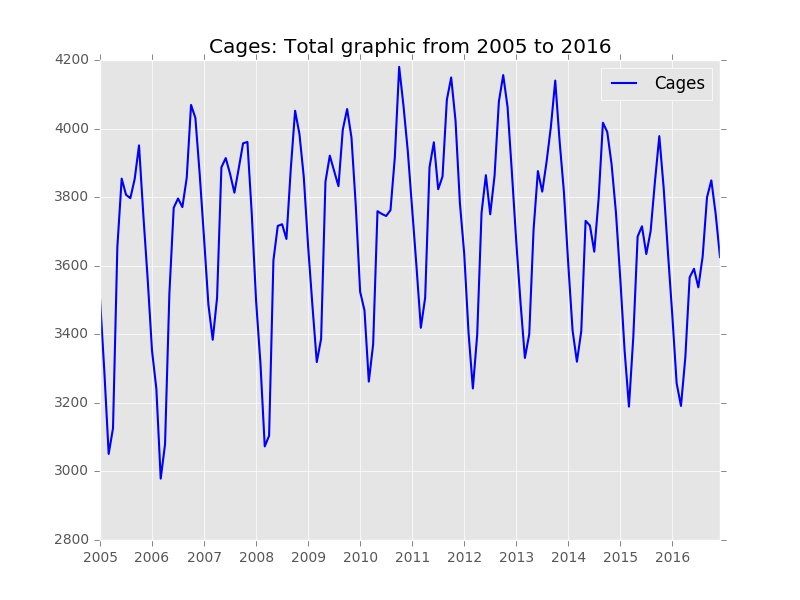
\includegraphics[width=0.9\textwidth]{Files/Cages_Total.jpg}
\caption{Total graphic about current input with total data from 2005 to 2016.}
\end{figure}
\end{minipage}


\newpage
\subsubsection{SIA section II: Single graphics for each year}

\textbf{Goal:}\\
Generate and display graphics about current input for each year from 2005 to 2016

\textbf{Requirements:}\\
- Data content: 144 values, 1 value for each month from 2005 to 2016

\textbf{Code implementation:}\\
During this section of the code was used "pandas" library for read the dataset.
\begin{lstlisting}
series2 = pd.read_csv("DATASET_DIRECTORY", 
	index_col=['Month'], 
	header=0, usecols=[0,1,2,3,4,5,6,7,8,9,10,11,12])
\end{lstlisting}

Then using the "pyplot" library has been possible to setup the plot of the input data.
\begin{lstlisting}
series2.plot()
\end{lstlisting}

Adding the title at the graphic that we are going to display.
\begin{lstlisting}
pyplot.title("Single year's graphic from 2005 to 2016")
\end{lstlisting}

There is the possibility to save the graphic like an image and/or display it.
\begin{lstlisting}
pyplot.savefig("OUTPUT_DIRECTORY", format="jpg")
pyplot.show()
\end{lstlisting}


\begin{minipage}{0.5\textwidth}
\textbf{Results:} \\
With this second part of the code has been reached the goal of displaying and save the graphics about the current input for each single year from 2005 to 2016, that looks like this example:
\end{minipage} \hfill
\begin{minipage}{0.45\textwidth}
\begin{figure}[H]
    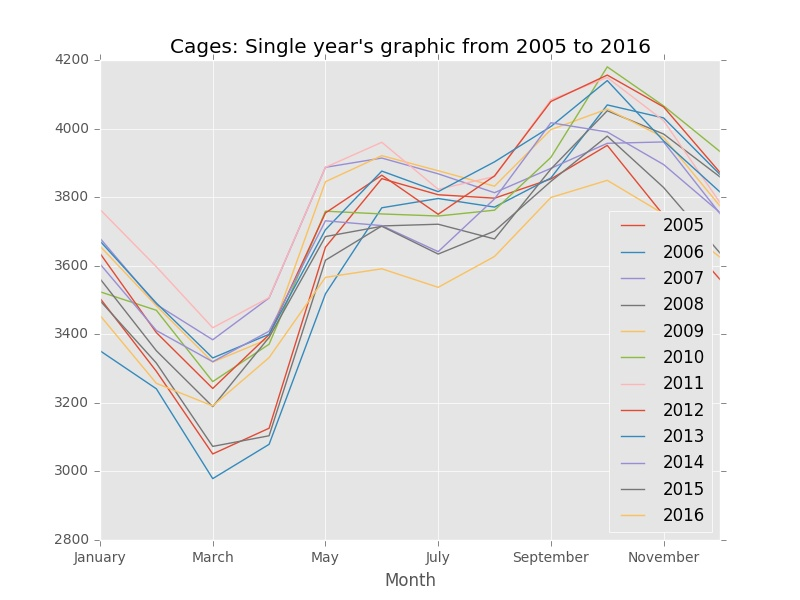
\includegraphics[width=0.9\textwidth]{Files/Cages_Years.jpg}
    \caption{Graphics for each single year of the input data from 2005 to 2016}
\end{figure}
\end{minipage}



\newpage
\subsubsection{SIA section III: Correlation matrix between years}

\textbf{Goal:}\\
Calculate the correlation coefficients between each single year from 2005 to 2016 of the current input and then display it with a correlation matrix.

\textbf{Requirements:}\\
- Data content: 144 values, 1 value for each month from 2005 to 2016

\textbf{Code implementation:}\\
During this section of the code was used "pandas" library for read the dataset.
\begin{lstlisting}
series3 = pd.read_csv("DATASET_DIRECTORY",
	 header=0, usecols=[1,2,3,4,5,6,7,8,9,10,11,12])
\end{lstlisting}

With the library "numpy" is possible to calculate the correlation coefficents between all the variables in the series just read.
\begin{lstlisting}
test = np.corrcoef(series3.values)
\end{lstlisting}

Setup the figure that will display the correlation matrix using the library "pypot".
\begin{lstlisting}
fig2 = pyplot.figure()
ax = fig2.add_subplot(111)
\end{lstlisting}

Creating the correlation matrix using the already calculated correlation coefficents.
\begin{lstlisting}
cax = ax.matshow(test, interpolation='nearest')
\end{lstlisting}

Settings for display the matrix in the right way, in particular for the values to display on both the axis x and y, in this case every single year from 2005 to 2016
\begin{lstlisting}
years = ["2005","2006","2007","2008","2009","2010",
	"2011","2012","2013","2014","2015","2016"]
x_pos = np.arange(len(years))
y_pos = np.arange(len(years))
pyplot.yticks(y_pos,years)
pyplot.xticks(x_pos,years)
\end{lstlisting}
\newpage
Adding a title to the graphic that we are going to display and also a bar that works like a legend for the colors of the matrix, allowing the reader to better understand the values reported inside the matrix.
\begin{lstlisting}
pyplot.title("Correlation between different years")
pyplot.colorbar(cax)
\end{lstlisting}

There is the possibility to save the correlation matrix like an image and/or display it.
\begin{lstlisting}
pyplot.savefig("OUTPUT_DIRECTORY", format="jpg")
pyplot.show()
\end{lstlisting}

\begin{minipage}{0.5\textwidth}
\textbf{Results:} \\
With this third part of the code have been calculated the correlation coefficients between each single year from 2005 to 2016 for each single inputs, saved the values in a document and then also displayed and saved the correlation matrix about it, that looks like this example:
\end{minipage} \hfill
\begin{minipage}{0.45\textwidth}
\begin{figure}[H]
    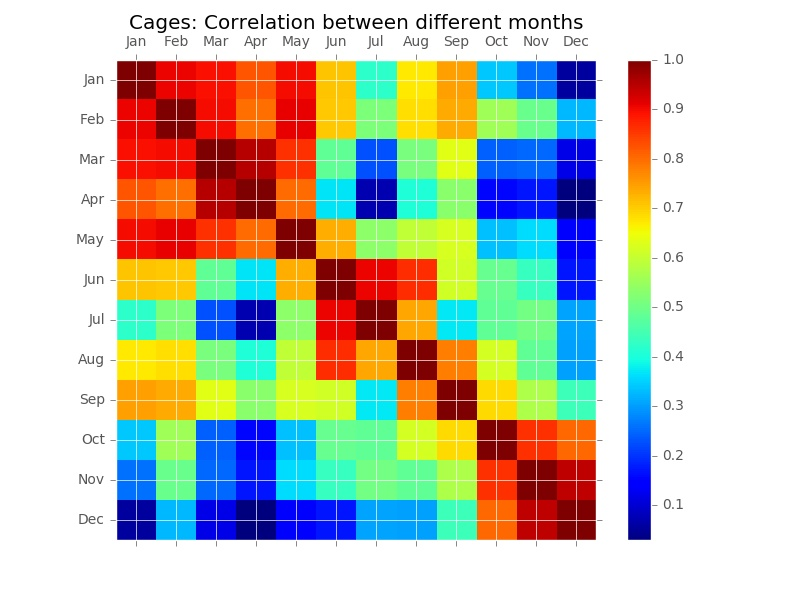
\includegraphics[width=0.9\textwidth]{Files/Cages_Months_Matrix.jpg}
    \caption{Correlation matrix between different months of the same input}
\end{figure}
\end{minipage}



\newpage
\subsubsection{SIA section IV: Correlation matrix between months}

\textbf{Goal:}\\
Calculate the correlation coefficients between each single month from 2005 to 2016 of the current input and then display it with a correlation matrix.

\textbf{Requirements:}\\
- Data content: 144 values, 1 value for each month from 2005 to 2016

\textbf{Code implementation:}\\
During this section of the code was used "pandas" library for read the dataset.
\begin{lstlisting}
series4 = pd.read_csv("DATASET_DIRECTORY", header=0, 
	usecols=[1,2,3,4,5,6,7,8,9,10,11,12])
\end{lstlisting}

With the library "numpy" is possible to calculate the correlation coefficents between all the variables in the series just read.
\begin{lstlisting}
test = np.corrcoef(series4.values)
\end{lstlisting}

Setup the figure that will display the correlation matrix using the library "pypot".
\begin{lstlisting}
fig2 = pyplot.figure()
ax = fig2.add_subplot(111)
\end{lstlisting}

Creating the correlation matrix using the already calculated correlation coefficents.
\begin{lstlisting}
cax = ax.matshow(test, interpolation='nearest')
\end{lstlisting}

Settings for display the matrix in the right way, in particular for the values to display on both the axis x and y, in this case every single months of the year.
\begin{lstlisting}
months = ["Jan","Feb","Mar","Apr","May","Jun",
	"Jul","Aug","Sep","Oct","Nov","Dec"]
x_pos = np.arange(len(months))
y_pos = np.arange(len(months))
pyplot.yticks(y_pos,months)
pyplot.xticks(x_pos,months)
\end{lstlisting}
\newpage
Adding a title to the graphic that we are going to display and also a bar that works like a legend for the colors of the matrix, allowing the reader to better understand the values reported inside the matrix.
\begin{lstlisting}
pyplot.title("Correlation between different months")
pyplot.colorbar(cax)
\end{lstlisting}

There is the possibility to save the correlation matrix like an image and/or display it.
\begin{lstlisting}
pyplot.savefig("OUTPUT_DIRECTORY", format="jpg")
pyplot.show()
\end{lstlisting}

\begin{minipage}{0.5\textwidth}
\textbf{Results:} \\
With this part of the code have been calculated the correlation coefficients between each single month from 2005 to 2016 of all the inputs and saved it in a document. Then has been also displayed and saved the correlation matrix about it, that looks like this example:
\end{minipage} \hfill
\begin{minipage}{0.45\textwidth}
\begin{figure}[H]
    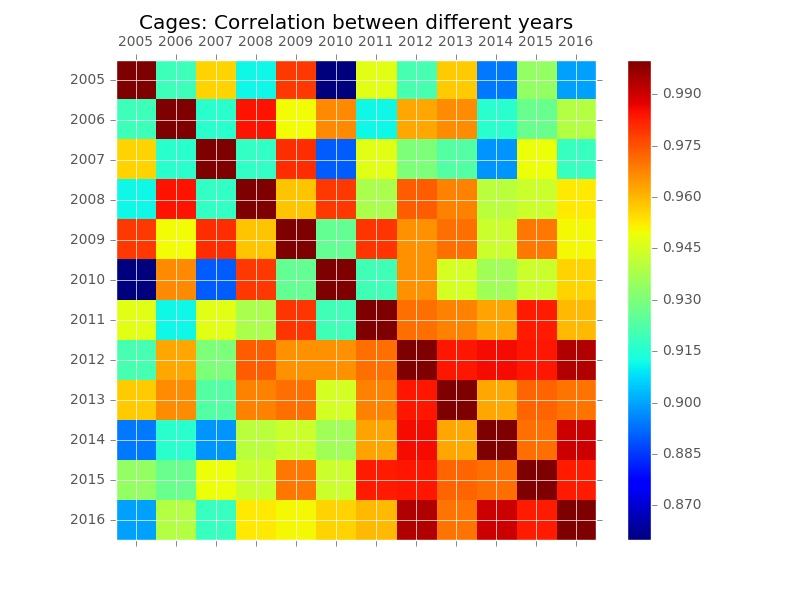
\includegraphics[width=0.9\textwidth]{Files/Cages_Years_Matrix.jpg}
    \caption{Correlation matrix between different years of the same input}
\end{figure}
\end{minipage}

\newpage
\subsubsection{SIA section V: Single and Total overview}

\textbf{Goal:}\\
Generate and display a single overview image for the current input.

\textbf{Requirements:}\\
- All the images that contain graphic about current input.

\textbf{Code implementation:}\\
create\_single\_overview() : this method will use the "Image" library for autogenerate a collage of the current input's graphics and save it like an overview image. The content of the params will basically decide how the "Current input overview image" will looks like.

It uses each single "current input overview image" of all the inputs and the "correlation matrix between all the inputs image" for combine them in a unique "total overview" and save it using the PDF format.

\begin{lstlisting}
listofimages=["CURRENT_INPUT_TOTAL_GRAPHIC",
            "CURRENT_INPUT_YEARS_MATRIX", 
            "CURRENT_INPUT_YEARS_GRAPHIC",
            "CURRENT_INPUT_MONTHS_MATRIX"]
           
create_single_overview(params1, listofimages)
create_single_overview(params2, listofimages)
\end{lstlisting}


The "create\_single\_overview" method has basically this structured, and then its configuration depends from the input data and from the preferences.
\begin{lstlisting}
def create_single_overview(cols, rows ,
			width, height, listofimages):
    thumbnail_width = width//cols
    thumbnail_height = height//rows
    size = thumbnail_width, thumbnail_height
    new_im = Image.new('RGB', (width, height))
    ims = []
    for p in listofimages:
        im = Image.open(p)
        im.thumbnail(size)
        ims.append(im)
    i = 0
    x = 0
    y = 0
    for col in range(cols):
        for row in range(rows):
            new_im.paste(ims[i], (x, y))
            i += 1
            y += thumbnail_height
        x += thumbnail_width
        y = 0
    new_im.save(SINGLE_OVERVIEW_IMAGE")
	new_im.show()
\end{lstlisting}

\textbf{Results:}
\begin{figure}[H]
	\centering
    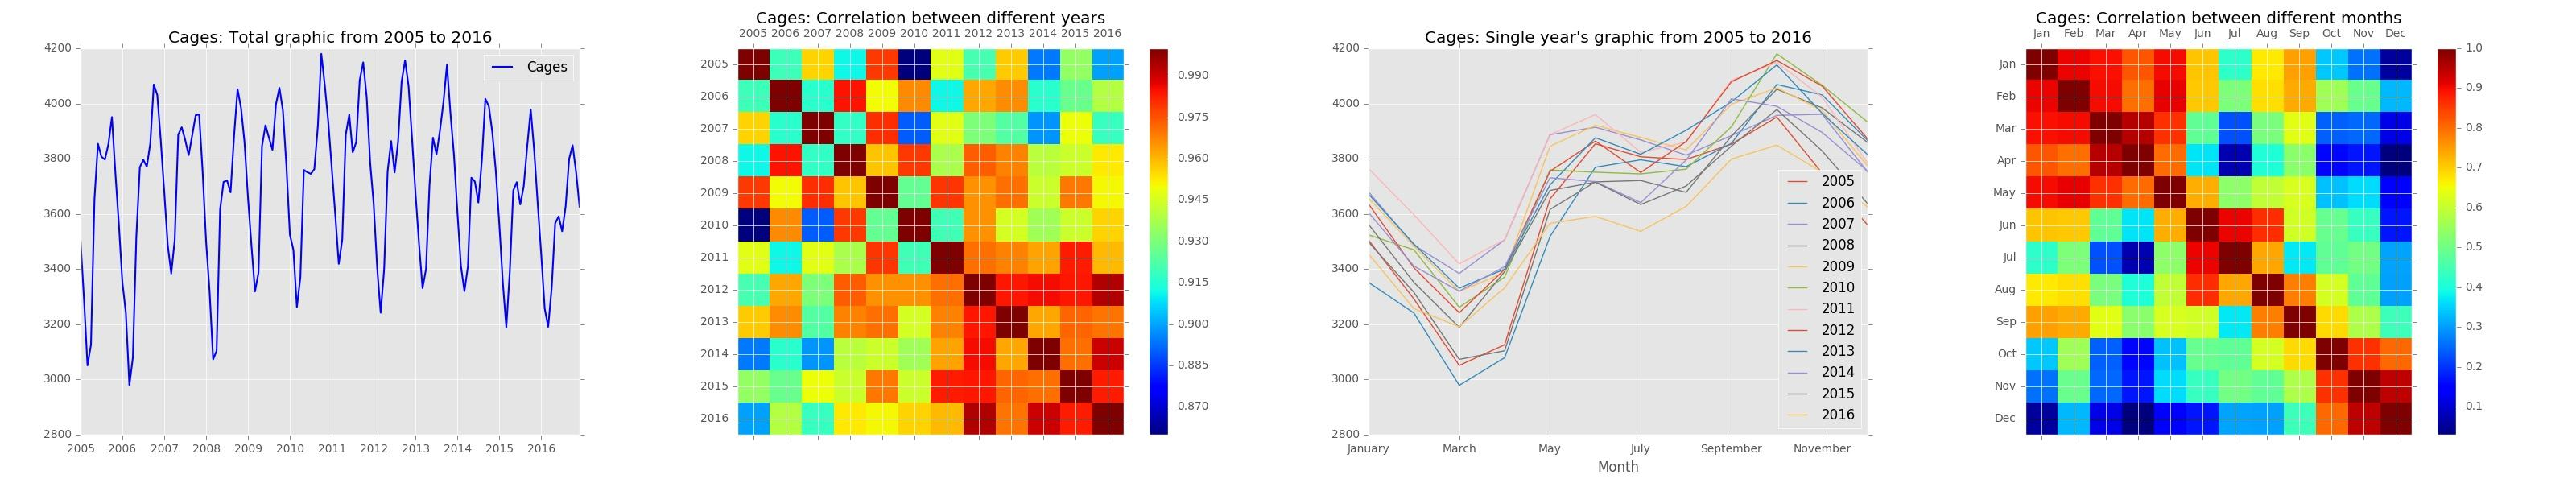
\includegraphics[width=1\textwidth]{Files/Cages_Overview.jpg}
    \caption{Example of "Single Input Overview Image"}
\end{figure}




\newpage
\subsection{Multiple Inputs Analyzer}
\subsubsection{MIA: Imported libraries}
The "pandas" library will be very useful for read the data from CSV dataset and setup the plot abut it.
\begin{lstlisting}
import pandas as pd
\end{lstlisting}

The "numpy" library it's used for mathematic purpose, such as calculating the correlation coefficent between two series.
\begin{lstlisting}
import numpy as np
\end{lstlisting}
 
The "pyplot" library it's used for basic graphic displaying and customization, easy to use but very efficent.
\begin{lstlisting}
import matplotlib.pyplot as pyplot
\end{lstlisting}

Also the library "sys" would be very useful for test and execute the program, mainly because it allows to input directly from terminal.
\begin{lstlisting}
import sys
\end{lstlisting}

\newpage
\subsubsection{MIA: Implementation}
\textbf{Goal:}\\
This analyzer is mainly used for show the correlation coefficent between the diffent inputs along the total period (from 2005 o 2016), that it will be important to have a general about which kind of relation there is between different inputs and how much strong it is.

\textbf{Requirements:}\\
- Input dataset: Total\_Dataset required, structure already reported here:
\hyperref[table: Total_Dataset]{Total Dataset}

\textbf{Code implementation:}\\
First of all, we are going to use the "pandas" library for read the dataset.
\begin{lstlisting}
series3 = pd.read_csv("TOTAL_DATASET_DIRECTORY", 
	index_col=['Input'], header=0)
\end{lstlisting}

Then with the library "numpy" is possible to calculate the correlation coefficents between all the variables just read above.
\begin{lstlisting}
test = np.corrcoef(series3.values)
\end{lstlisting}

Setup the figure that will display the correlation matrix using the library "pyplot".
\begin{lstlisting}
fig2 = pyplot.figure()
ax = fig2.add_subplot(111)
\end{lstlisting}

Creating the correlationg matrix using the already calculated correlation coefficents.
\begin{lstlisting}
cax = ax.matshow(test, interpolation='nearest')
\end{lstlisting}

Settings for display the matrix in the right way, in particular for the values to display on both the axis x and y, in this case every single input.
\begin{lstlisting}
inputs = ["Cages", "Feed", "Number", "Restock",
	"Local", "Withdr", "Biomass", "Price"]
x_pos = np.arange(len(inputs))
y_pos = np.arange(len(inputs))
pyplot.yticks(y_pos,inputs)
pyplot.xticks(x_pos,inputs)
\end{lstlisting}

Adding a title to the graphic that we are going to display and also a ba that works like a legend for the colors of the matrix, allowing the reader to better understand the values reported inside the matrix.
\begin{lstlisting}
pyplot.title("Correlation between different inputs 
		about data from 2005 to 2016")
pyplot.colorbar(cax)
\end{lstlisting}

In the end, using again the library "pyplot", there is the possibility to save the correlation matrix graphic like an image and/or display it.
\begin{lstlisting}
pyplot.savefig("OUTPUT_DIRECTORY")
\end{lstlisting}

\begin{lstlisting}
series = pd.read_csv("TRENDLINES_VALUES_DOCUMENT",
	 header=0, usecols=["Norm Ang Coeffs"])
series.plot(kind="barh")
pyplot.savefig("OUTPUT_DIRECTORY")

create_total_overview()
\end{lstlisting}

\begin{lstlisting}
pyplot.show()
\end{lstlisting}




\textbf{Results:} \\

\begin{figure}[H]
	\centering
    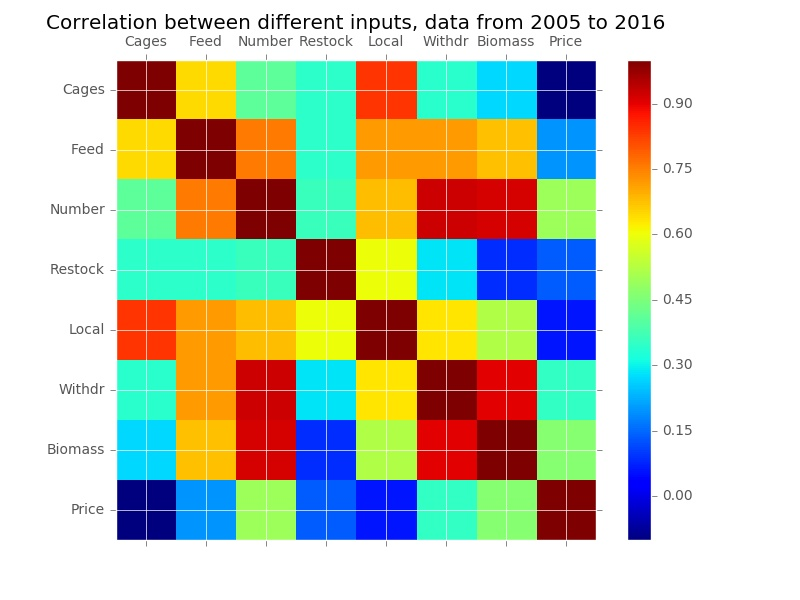
\includegraphics[width=0.75\textwidth]{Files/Total_Dataset_Years_Matrix.jpg}
    \caption{Correlation matrix between different inputs with data from 2005 to 2016.}
\end{figure}

\begin{figure}[H]
	\centering
    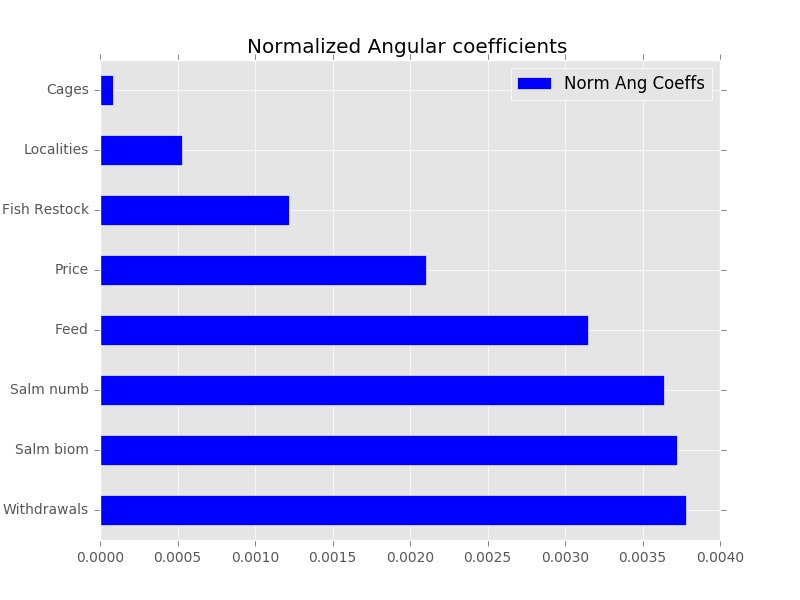
\includegraphics[width=0.75\textwidth]{Files/Norm_Ang_Coeffs.jpg}
    \caption{Normalized angular coefficients of each input's trendline.}
\end{figure}


\newpage
\section{Extract information from data}
 % Experiment 1

\part{Experiment 2: Values prediction system}
\section{3th Phase: Data prediction system implementation}
\section{4th Phase: Prediction results displaying}
 % Experiment 2




 
%\chap{Results}



 

%----------------------------------------------------------------------------------------
%	THESIS CONTENT - APPENDICES
%----------------------------------------------------------------------------------------

\appendix % Cue to tell LaTeX that the following "chapters" are Appendices

% Include the appendices of the thesis as separate files from the Appendices folder
% Uncomment the lines as you write the Appendices

\chap{An Appendix}
%\include{Appendices/AppendixB}
%\include{Appendices/AppendixC}

%----------------------------------------------------------------------------------------
%	BIBLIOGRAPHY
%----------------------------------------------------------------------------------------

\printbibliography[heading=bibintoc]

%----------------------------------------------------------------------------------------

\end{document}  
